
\chapter{Installing and Configuring Softwares}

In this task, you are required to install the tools you've already been familiar
with (at least heard about).

\textbf{Important notes:} This might be the hardest part of your Homework 0,
since installation of the same software on different platforms differs a lot,
which means we could not show you detailed steps for each platform. Instead, we
will provide you with links for the installation instructions for you to follow,
and we have created three forums for you to discuss Windows/Linux/Mac platform
related issues. We will try our best to help you solve whatever problems you
might have, but we also encourage you, the experts in any of these platforms, to
work with us to answer the questions from your classmates. You can find the
discussion boards at \url{http://blackboard.andrew.cmu.edu}, and select the
course, then the \textbf{Tools} and \textbf{Discussion Board}.


\section{Installing JDK}

If you have the latest JDK 6 installed\footnote{You should check out the latest version at \url{http://www.oracle.com/technetwork/java/javase/downloads/index.html} as the version number grows really fast}, you could skip this task.

We assume you have experience in Java programming, but we still need to clarify the Java environment for the course. If you don't have any Java experience, probably you need to look for a Java textbook. It might also be fine if you think you have tons of experience in programming in C++/C\# and you feel confident to learn Java by just reading others' codes and guessing their meanings. It's up to you!

\begin{enumerate}
\item Visit \url{http://www.oracle.com/technetwork/java/javase/downloads/index.html}, and choose the platform you are using to download JDK 6 SE 35\footnote{By the date of August 31, 2012}.

\begin{qa}
\item[Q1] Can I just install JRE instead of JDK?
\item[A1] No.
\item[Q2] Can I install OpenJDK instead of SunJDK (or OracleJDK)?
\item[A2] Sure, you can. But be aware that sometimes only binary files (aka JRE) are installed under a folder named \texttt{openjdk-\emph{version}}, rather than \texttt{openjre-\emph{version}}, which is a bit confusing.
\item[Q3] Can I install JDK 7, 5 or older versions?
\item[A3] You are not recommended to install JDK 7, since you have to modify the Maven pom file to compile your project, and the cluster that we will run and test your components does not have JDK 7 set up yet. But it would be fine (theoretically) if you have just JDK 5 installed, but it is still not recommended. Versions older than 5 should be completely avoided.
\item[Q4] Can I use an earlier version of JDK 6 (e.g., 6u4)?
\item[A4] It may not put you in a trouble most of time, but in some rare cases, we did find an exception was thrown due to a bug not in our code but in the runtime environment. Therefore, we recommend you to upgrade your JDK 6 to the latest version.
\end{qa}

\item Install JDK from the executable file if available, and set PATH manually (if you are using a Windows machine). The Java installation page (at \url{http://www.oracle.com/technetwork/java/javase/index-137561.html}) might be useful to you.
\end{enumerate}


\section{Installing Git}

If you have Git installed, you can skip this task.

You will not need Git (specifically, execute Git goals from command line) in most cases, because we will have EGit (the Git plug-in for Eclipse) installed. But sadly, there is a case you have to install the Git, when the Maven plug-in for Eclipse (aka m2e) does need Git (not EGit) and the SCM URI you specified to execute Git commands. (Don't know what SCM is? Probably you need to go back to the previous task.)

\begin{enumerate}
\item Visit \url{http://git-scm.com/downloads} to download Git.
\item You can refer to the Pro Git book for how to install Git for different platforms (at \url{http://git-scm.com/book/en/Getting-Started-Installing-Git}), and how to set up Git (at \\\url{http://git-scm.com/book/en/Getting-Started-First-Time-Git-Setup}).
\end{enumerate}


\section{Performing a Maven Release}

In the last task, you will need to submit your Java code by performing a release
of your code. But remember that Maven release plug-in will check if all the
changes you have made have been checked into the remote repository (i.e. GitHub
in our case). So, let's perform a git-commit and a git-push.

\begin{enumerate}

\begin{figure}
\hspace{-1em}
\begin{minipage}{0.5\textwidth}
\centering
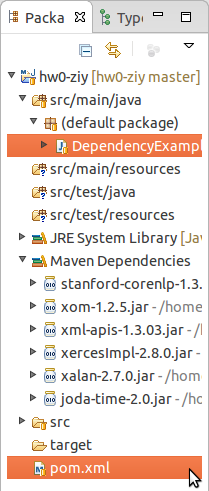
\includegraphics[scale=0.3]{simple-code-05-commit}
\caption{Performing a git-commit/push before preparing a release\label{simple-code-05-commit}}
\end{minipage}
\hfill
\begin{minipage}{0.5\textwidth}
\centering
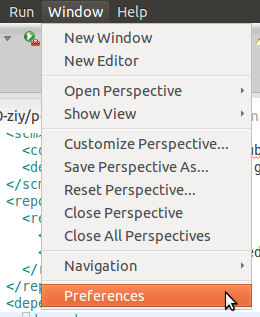
\includegraphics[scale=0.3]{submit-01-preference}
\caption{Starting to add an external Maven executable\label{submit-01-preference}}
\end{minipage}
\hspace{-1em}
\end{figure}

\item Similar to what you did earlier, you execute git-commit and git-push to
the project, and you could see the ``greater than'' symbol disappears and a
``master'' label is attached to project path, which means you are successful
with your git-commit and git-push.

\begin{figure}
\hspace{-2em}
\begin{minipage}{0.5\textwidth}
\centering
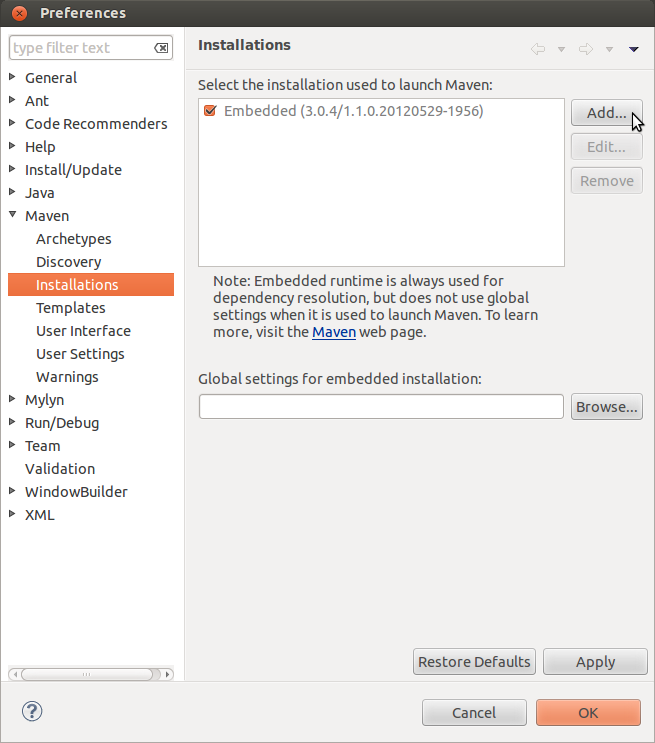
\includegraphics[scale=0.3]{submit-02-add-maven}
\caption{Adding another Maven executable\label{submit-02-add-maven}}
\end{minipage}
\hfill
\begin{minipage}{0.5\textwidth}
\centering
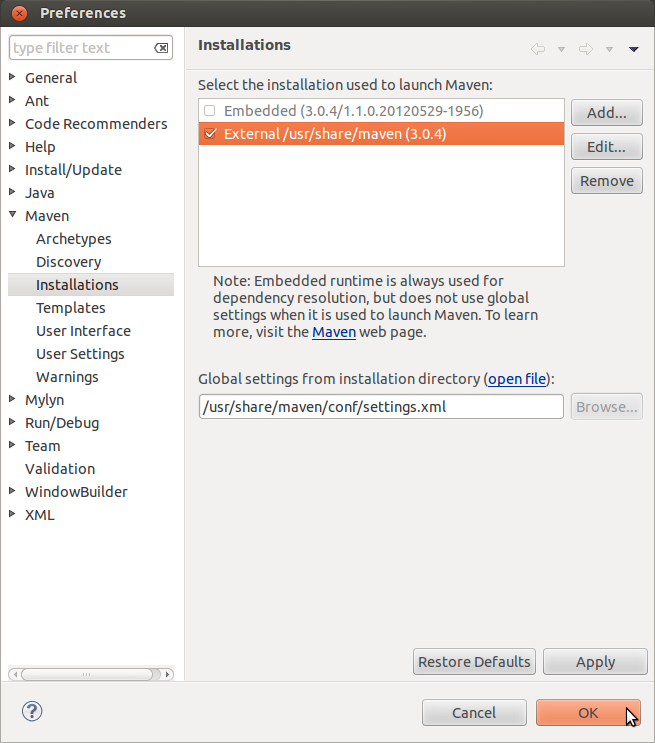
\includegraphics[scale=0.3]{submit-03-add-maven-done}
\caption{Viewing the added external Maven\label{submit-03-add-maven-done}}
\end{minipage}
\hspace{-2em}
\end{figure}

\item Sometimes, the embedded Maven runtime from m2e cannot be succesfully
executed to perform a release goal. Therefore, we should add the externally
installed Maven runtime into the Eclipse. Click \textbf{Window} (or
\textbf{Edit}) $\rightarrow$ \textbf{Preferences} (see Figure
\ref{submit-03-add-maven-done}).

\item Select \textbf{Maven} $\rightarrow$ \textbf{Installations}. You will see
the ``Embedded'' runtime (as shown in Figure \ref{submit-02-add-maven}). Click
\textbf{Add\ldots} to locate the installation path of your Maven runtime.

\item Then, you could see an ``External'' runtime in the installation lists. See
Figure \ref{submit-03-add-maven-done}.

\begin{figure}
\centering
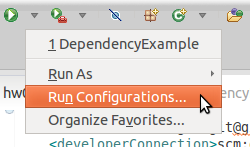
\includegraphics[scale=0.3]{submit-04-run-config}
\caption{Getting ready for a release\label{submit-04-run-config}}
\end{figure}

\item Now you can execute a Maven goal within Eclipse (of course, you can also
do that outside Eclipse from command line). Click the down-arrow next to the
\textbf{Run} button, and select \textbf{Run Configurations\ldots}. See Figure
\ref{submit-04-run-config}.

\begin{figure}
\centering
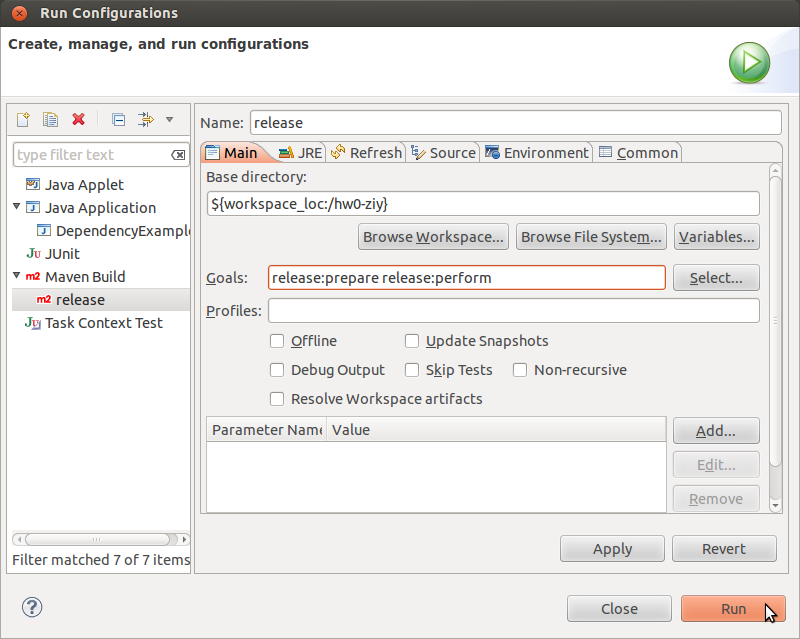
\includegraphics[scale=0.3]{submit-05-run-config-done}
\caption{Configuring Maven goal\label{submit-05-run-config-done}}
\end{figure}

\item In the ``Run Configurations'' window, double-click \textbf{Maven Build} to
create a new Maven goal. See Figure \ref{submit-05-run-config-done}. Rename your
run configuration name as ``release'' (optional), and click \textbf{Browse
Workspace\ldots} to select your project, and type in your goals as follows:

\begin{verbatim}
release:prepare release:perform
\end{verbatim}

This actually defines two goals ``release:prepare'' and ``release:perform''. As
you will probably encounter tons of errors during this step, we should review
some details of the Maven release.

The Maven
guide\footnote{\url{https://maven.apache.org/guides/mini/guide-releasing.html}}
tells us what is happening behind these two goals:

\begin{quote}
The release:prepare goal will:

\begin{enumerate}
\item Verify that there are no uncommitted changes in the workspace.
\item Prompt the user for the desired tag, release and development version
names.
\item Modify and commit release information into the pom.xml file.
\item Tag the entire project source tree with the new tag name.
\end{enumerate}

The release:perform goal will:

\begin{enumerate}
\item Extract file revisions versioned under the new tag name.
\item Execute the maven build lifecycle on the extracted instance of the
project.
\item Deploy the versioned artifacts to appropriate local and remote
repositories.
\end{enumerate}
\end{quote}

If the goals are not executed sucessfully, a relatively useful message will be
printed out to console to help you discover where the problem is.

\begin{figure}
\centering
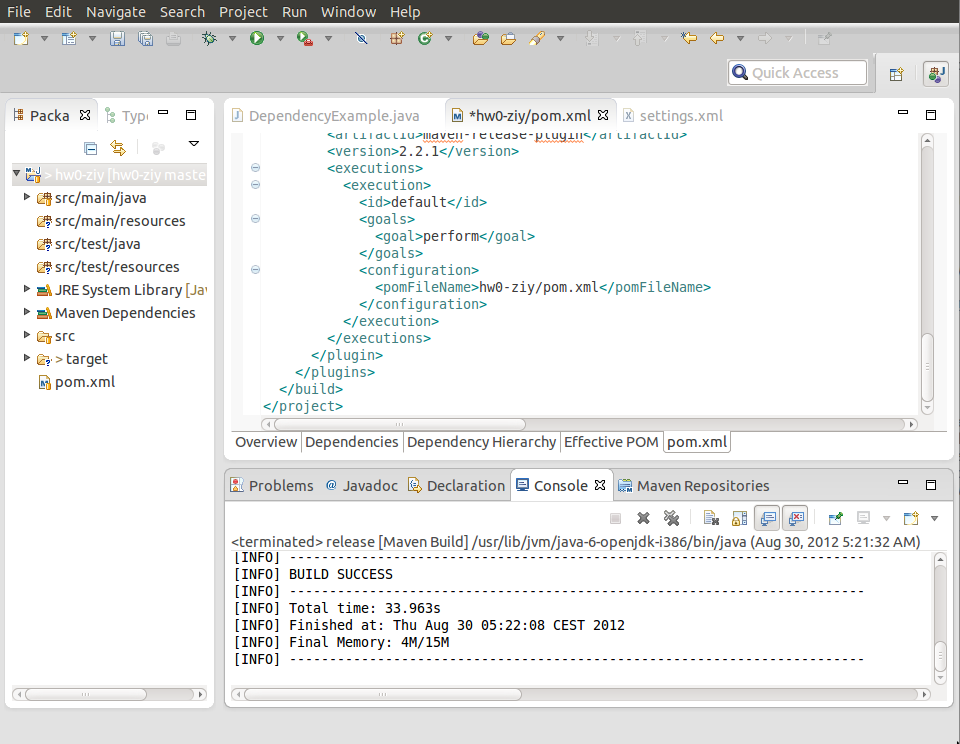
\includegraphics[scale=0.3]{submit-06-release}
\caption{A successful release!\label{submit-06-release}}
\end{figure}

\item Finally after you fixed all the problems (if any), you could see the very
pleasant ``BUILD SUCCESS'' message in the console (as shown in Figure
\ref{submit-06-release}), which means you've done with your Homework 0!
Congratulations!

\begin{qa}

\item[Q1] The ``release:prepare'' goal could be executed successfully, but there
was an error during ``release:perform''. How can I start all over
again?\footnote{Reported by Kartik Mandaville.}

\item[A1] A successful ``prepare'' with an unsuccessful ``perform'' always leads
to a very subtle situation. Sometimes, you can try to execute a
``release:rollback'' Maven goal to revert to the previous status, or you are try
to manually delete the \verb|release.properties| file under your project
diretory, and make sure you are now working on a SNAPSHOT version. (You can
check your version from Maven POM Editor, and you have an opened Maven POM
Editor, be sure to close it and open it again since it will not be automatically
refreshed after you execute a Maven goal.) If it is no longer a SNAPSHOT
version, you should modify the \textbf{Version} field to something like
``0.0.2-SNAPSHOT'' (without quotes). You might want to refer to
\url{http://maven.apache.org/guides/mini/guide-releasing.html} about the details
of the release process.

\item[Q2] The process hangs forever during Maven ``release:prepare'' executing a
``git push'' command, in other words, it doesn't terminate or produce any
further useful information. What should I do?

\item[A2] We are sure there is some bug with the plugin related to this issue.
But there still some workarounds to consider.

\begin{enumerate}
\item If you generate a public key with a passphrase (i.e., you typed in
something before you pressed \textbf{Enter}), then try to regenerate another
public key following the same instruction and paste it to GitHub.
\item Try to log back into GitHub to see if your email address has been
verified.
\item Turn to command line to execute Maven goal by typing
\verb|mvn release:prepare release:perform| from the project directory to see
if it terminates automatically or still hangs there forever.
\item Try to find the last command in the log message shown in the console
(e.g., \verb|git push ... master:master|), and directly type in the same command
in the command line to see if additional verification (e.g., adding a host to
\verb|known_host| list) is required.
\end{enumerate}

\item[Q3] What if I find some bugs after it has been released? How can I
resubmit my code?

\item[A3] You can look at the ``Overview'' tab in the Maven POM Editor for your
pom.xml file. The version should be ``0.0.2-SNAPSHOT'', which indicates a
previous version has been generated. Now, you could redo this task (git-commit,
git-push, run Maven goals) to release the version 0.0.2. We will evaluate your
code based on the latest release.

\item[Q4] How could I check if my submission is successful?

\item[A4] First of all, don't worry about it, even if by the deadline, we
haven't received your submission, we will notify you, and help you check what
the problem may be before you start Homework 1.

If you want to check your submission, you can go to
\url{http://mu.lti.cs.cmu.edu:8081/nexus/index.html} back again, and log in with
your password, go to \textbf{View/Repositories} $\rightarrow$
\textbf{Repositories} on the left, then click \textbf{Course Releases} on the
right, unfold directories along the groupId path, and if you see your artifact
at the end, then you've done!

\end{qa}

\end{enumerate}


\section{Eclipse (Git, Maven plug-ins integrated)}

If you have an Eclipse IDE for Java Developers with version $\ge$ 3.7, you could
probably skip this task. But if you are stuck in a situation where you were told
Eclipse is missing a plug-in, you might want to return to this section. If you
have other packages (Eclipse Classic or Eclipse for Java EE Developers), please
do not skip this task.

\begin{enumerate}

\item Download Eclipse IDE for Java Developers 4.2 at
\url{http://www.eclipse.org/downloads/packages/eclipse-ide-java-developers/junor}.

\begin{qa}

\item[Q1] Can I use an older version of Eclipse?

\item[A1] You can try to use an older version, but some plug-ins (e.g., m2e)
might complain about the Eclipse version if it is older than 3.7.

\item[Q2] Can I use other Eclipse packages?

\item[A2] Eclipse IDE for Java Developers includes almost all the Eclipse
components (jdt, EGit, m2e, and so on) we need for this course. You could also
work with other packages, e.g., Eclipse IDE for Jave EE Developers or Eclipse
Classics, and as they don't come with such plugins by default, you have to
install these plug-ins all by yourself.

\end{qa}

\item Install Eclipse by simply uncompressing the downloaded package.

\begin{figure}[t]
\centering
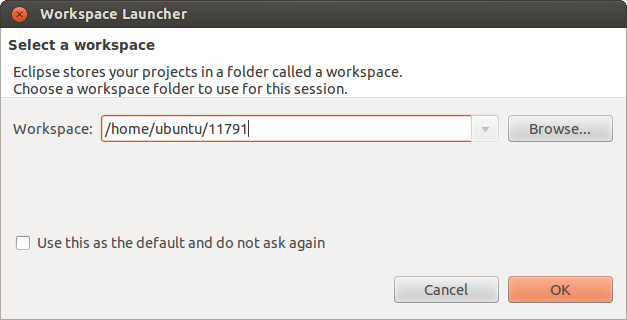
\includegraphics[scale=0.3]{eclipse-01-login}
\caption{Eclipse choose workspace\label{eclipse-01-login}}
\end{figure}

\item Use the default workspace path or create your own workspace, as shown in
Figure \ref{eclipse-01-login}. And finally, we could see the Eclipse Welcome
view at the end of workspace initialization. See Figure
\ref{eclipse-02-welcome}.

\begin{figure}[t]
\centering
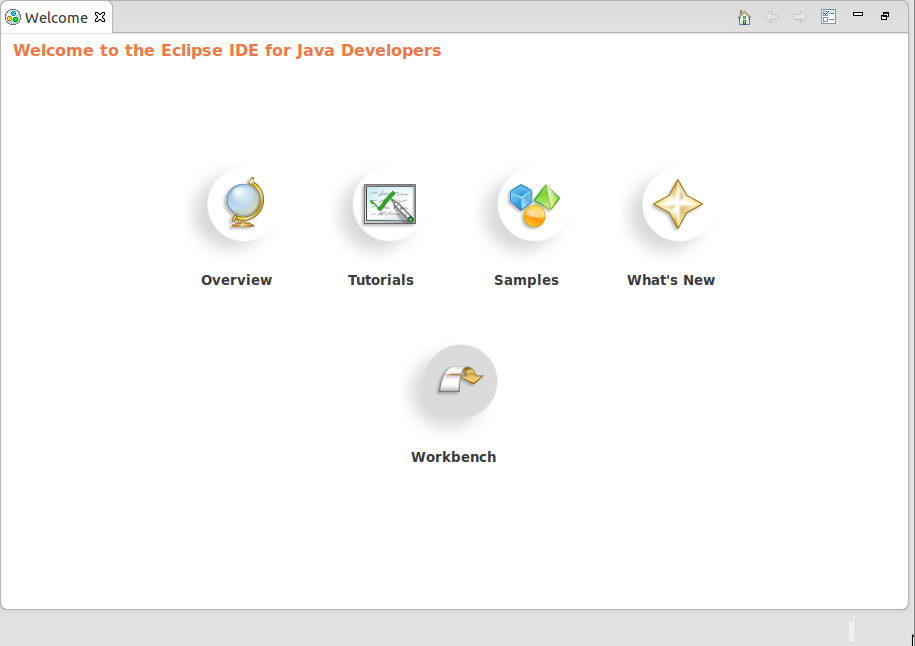
\includegraphics[scale=0.3]{eclipse-02-welcome}
\caption{Eclipse Welcome view\label{eclipse-02-welcome}}
\end{figure}

\end{enumerate}


That's the start of your developement. From now on, everthing will become less
platform specific, and we will show you how to configure the workspace, create
your Maven project and release it in the rest of the homework.


\section{A Little Configuration}

\subsection{Letting m2e know your password}

\begin{enumerate}

\item Click \textbf{Edit} (or \textbf{Window} depending on your OS)
$\rightarrow$ \textbf{Preferences}, and choose \textbf{Maven} $\rightarrow$
\textbf{User Settings}, and find the default Maven setting path for your system.
See Figure \ref{eclipse-03-maven-setting}.

\item Create the \verb|settings.xml| file at the given directory, and copy the
text in Listing \ref{settings} into the file, which will store your ID and
passwords. Remember to replace \verb|ID| and \verb|PASSWORD| with your personal
Maven project repository account we provide you, and also don't upload this file
to any remote repository or share it with others.

\item Go back to \textbf{Edit} (or \textbf{Window}) $\rightarrow$
\textbf{Preferences}, and choose \textbf{Maven} $\rightarrow$ \textbf{User
Settings} again, you will see the plugin could find the setting file you
specified (see Figure \ref{eclipse-04-maven-setting-back}).
% and click \textbf{Update settings}. You will be able to see the repository is
% now being refreshed.

\begin{figure}[t]
\hspace{-3em}
\begin{minipage}{0.5\textwidth}
\centering
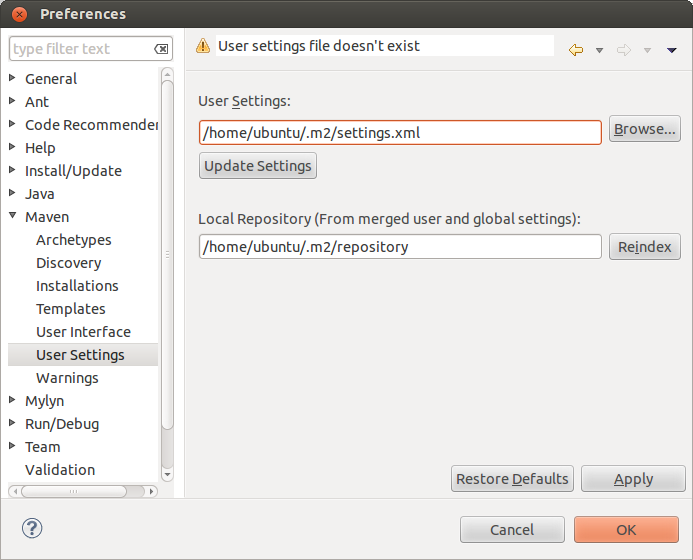
\includegraphics[scale=0.3]{eclipse-03-maven-setting}
\caption{Eclipse maven user profile setting\label{eclipse-03-maven-setting}}
\end{minipage}
\hfill
\begin{minipage}{0.5\textwidth}
\centering
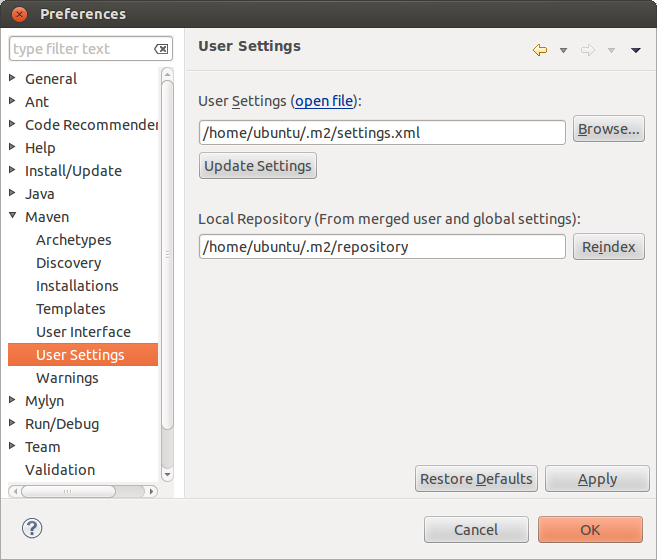
\includegraphics[scale=0.3]{eclipse-04-maven-setting-back}
\caption{Eclipse maven user profile setting\label{eclipse-04-maven-setting-back}}
\end{minipage}
\hspace{-3em}
\end{figure}

\lstinputlisting[language=XML,float,linewidth=1.1\textwidth,caption=Configuring settings.xml,label=settings]{settings.xml}

\end{enumerate}

\subsection{Importing Apache UIMA code style template}

To development a software as a team, members should always adopt the same code
conventions to improve the readability and maintainability of the project. We
suggest you to view the \emph{Code Conventions for the Java Programming
Language} at \url{http://www.oracle.com/technetwork/java/codeconv-138413.html},
which was published from Oracle. For our course homeworks, you are required to
adopt a set of more specific coding conventions from Apache UIMA project.
Details can be found at \url{http://uima.apache.org/codeConventions.html}. At
the bottom of the page, you could find a link to download the Eclipse code style
template\footnote{\url{http://uima.apache.org/downloads/ApacheUima_EclipseCodeStylePrefs.xml}}.

\begin{enumerate}
\item Download the template and save it in your local filesystem.
\item Click \textbf{Window} $\rightarrow$ \textbf{Preferences}, then go to \textbf{Java} $\rightarrow$ \textbf{Code Style} $\rightarrow$ \textbf{Formatter}, and click \textbf{Import\ldots}. 
\end{enumerate}

Remember before you finish editing a Java file, press \textbf{Ctrl+Shift+F} to
perform an automatic code formation.

Another optional but useful tool for you to check your code style is the Eclipse
Checkstyle plug-in. You can learn how to download and install the plug-in at
\url{http://eclipse-cs.sourceforge.net/}.

